\documentclass[12pt,a4paper]{article}

\usepackage{amsmath,amscd,amsbsy,amssymb,latexsym,url,bm,amsthm}
\usepackage{epsfig,graphicx,subfigure}
\usepackage{enumitem,balance}
\usepackage{wrapfig}
\usepackage{mathrsfs, euscript}
\usepackage[usenames]{xcolor}
\usepackage{hyperref}
\usepackage{multicol}

\theoremstyle{definition}

\newtheorem{theorem}{Theorem}
\newtheorem{lemma}[theorem]{Lemma}
\newtheorem{proposition}[theorem]{Proposition}
\newtheorem{corollary}[theorem]{Corollary}
\newtheorem{exercise}{Exercise}[section]
\newtheorem*{solution}{Solution}

\numberwithin{equation}{section}
\numberwithin{figure}{section}

\renewcommand{\thefootnote}{\fnsymbol{footnote}}

\newcommand{\postscript}[2]
 {\setlength{\epsfxsize}{#2\hsize}
  \centerline{\epsfbox{#1}}}

%changing 1.5 will give you different space between lines.
\renewcommand{\baselinestretch}{1.0}

\setlength{\oddsidemargin}{-0.365in}
\setlength{\evensidemargin}{-0.365in}
\setlength{\topmargin}{-0.3in}
\setlength{\headheight}{0in}
\setlength{\headsep}{0in}
\setlength{\textheight}{10.1in}
\setlength{\textwidth}{7in}

\begin{document}

\noindent\framebox[\linewidth]{\shortstack[c]{
\Large{\textbf{Lab05-Numbering Programs}}\vspace{1mm}\\
CS363-Computability Theory, Xiaofeng Gao, Spring 2016}}
\begin{center}
\footnotesize{\color{red}$*$ Please upload your assignment to FTP or submit a paper version on the next class}

\footnotesize{\color{red}$*$ If there is any problem, please contact: nongeek.zv@gmail.com }

\footnotesize{\color{blue}$*$ Name:Wenhao Zhu \quad StudentId: 5130309717 \quad Email: weehowe.z@gmail.com}
\end{center}


\begin{enumerate}%[topsep=0pt, partopsep=0pt, itemsep=2pt,parsep=2pt]
  \item Show that there is a total computable function $k$ such that for each $n$,
    \begin{enumerate}
      \item $k(n)$ is an index of the function $\lfloor\sqrt[n]{x}\rfloor$.
      \item $W_{k(n)}^{(m)}=\{(y_{1},\ldots,y_{m}):y_{1}+y_{2}+\ldots+y_{m}=n\}$ ($m\geq 1$).
      \item $E_{k(n)}=W_n$.
    \end{enumerate}
    \begin{solution}
      (a)Let $P_{m}$ be the program corresponding to $f_{P_{m}}(x)=\lfloor\sqrt[n]{x}\rfloor$\\
      then the $P_{m}$ can be describe as 1)keep calculating $i^{n}$, where i grow up 2)when the first $i^{n} > x$, stop 3)the result is $(i-1)$. So apparently we can decide the $P_{m}$ therefore by the Church's Thesis, $k(n)$ is computable.\\
      (b) $k(n)$ is the index of the function that will terminate $\iff \sum\limits_{i=0}^{m}{y_{i}} = n$\\
      So the corresponding $P_{k(n)}$ can check the input satisfy the condition. If not it will turn into a endless loop.\\
      By the Church's Thesis, the $k(n)$ is computable.\\
      (c) $f_{P_{k(n)}}(x)$ is the inverse function of the $f_{P{n}}$, $k(n)$ is apparently computable.      
    \end{solution}

  \item
  \begin{enumerate}
    \item Find $P_{1028}$. Distinguish what are $\phi_{1028}(x)$ and $\phi_{1028}^{(n)}(x_1,\cdots,x_n)$ and their corresponding $W_{1028}(x)$, $E_{1028}(x)$ and $W^{(n)}_{1028}(x)$, $E^{(n)}_{1028}(x)$;
    \begin{solution}
    $ $\\
    $P_{1028} = 2^{10} + 2^2$, so we can know that $a_1 = 2, a_2 = 7$.
    Therefore, the instructions are T(1,1) and J(1,1,2).
    $\phi_{1028}(x) = 1, W_{1028}(x) = N, E_{1028}(x) = {1}.$
    \end{solution}
    \item Let $P$ be the program J(1,2,4), Z(1), S(1). Calculate $\gamma(P)$.
    \begin{solution} 
    $ $ \\
    $ \beta(J(1,2,4)) = 4\zeta(1,2,4) + 3 = 4\pi(\pi(0,1),3) + 3  = 111 $ \\
    $ \beta(Z(1)) = 0 $\\
    $ \beta(S(1)) = 1 $\\
    Thus, $\gamma(P) = 2^{111} + 2^{112} + 2^{114} - 1$
    \end{solution}
  \end{enumerate}
\item

\begin{enumerate}
\item (Cantor) Show that the set of all functions from $\mathbb{N}$ to $\mathbb{N}$ is not denumerable.
\begin{proof}
Define $\mathcal{F}$ as all the functions maps $\mathbb{N}$ to $\mathbb{N}$. Let $f_0$, $f_1$, $f_2$, . . . be any
sequence of elements of $\mathcal{F}$ and by Cantor's Diagonal Method, we can define $f \in  \mathcal{F}$ by: \\
\begin{displaymath}
f(i) = \left\{ \begin{array}{ll}
f_i(i)+1 & \textrm{if $f_i(n)$ is defined}\\
0 & \textrm{otherwise} 
\end{array} \right.
\end{displaymath}
By construction $f(i) \ne f_i(n)$, so $f \ne f_i $ ( for any $i \in \mathbb{N}$ ), thus the set of all functions from $\mathbb{N}$ to $\mathbb{N}$ is not denumerable.
\end{proof}
\item Show that the set of all non-computable total functions from $\mathbb{N}$ to $\mathbb{N}$ is not denumerable.
\begin{proof}
Define $\mathcal{F}$ as all non-computable total functions maps $\mathbb{N}$ to $\mathbb{N}$. Let $f_0$, $f_1$, $f_2$, . . . be any
sequence of elements of $\mathcal{F}$, and these functions can be derived by previous problem, by Cantor's Diagonal Method, we can define $f \in  \mathcal{F}$ by: \\
\begin{displaymath}
f(i) = \left\{ \begin{array}{ll}
f_i(i)+a(i)+1 & \textrm{if $f_i(n)$ is defined}\\
a(i) & \textrm{otherwise} 
\end{array} \right.
\end{displaymath}
By construction $f(i) \ne f_i(n)$, so $f \ne f_i $ ( for any $i \in \mathbb{N}$ ), thus the set of all non-computable total functions from $\mathbb{N}$ to $\mathbb{N}$ is not denumerable.
\end{proof}
\end{enumerate}

\item Alternative Selection of $\pi$

  \begin{minipage}[t]{0.68\linewidth}
  The $\pi$ function where $\pi(x,y)=2^x (2y+1)-1$ can enumerate linearly all pairs of natural numbers $ (x,y) \in \mathbb{N}\times \mathbb{N}$. However, it does not generate a trace in the first quadrant of the plane. Correspondingly, instead of applying this $\pi$ function, we can define an alternative bijection $\pi'$, such that $\pi': \mathbb{N}\times \mathbb{N} \rightarrow \mathbb{N}$ and it grows horizontally and vertically according to the right figure. Thus we have:

    \vspace{1mm}
  $\pi'(0,0)=0$, $\pi'(0,1)=1$, $\pi'(1,0)=2$,

  $\pi'(1,1)=3$, $\pi'(0,2)=4$, $\pi'(1,2)=5$, 

    $\pi'(2,0)=6$, $\pi'(2,1)=7$, $\pi'(2,2)=8$, etc.
  \end{minipage}
  \hspace{1mm}
  \begin{minipage}[t]{0.32\linewidth}
  \vspace{0pt}
    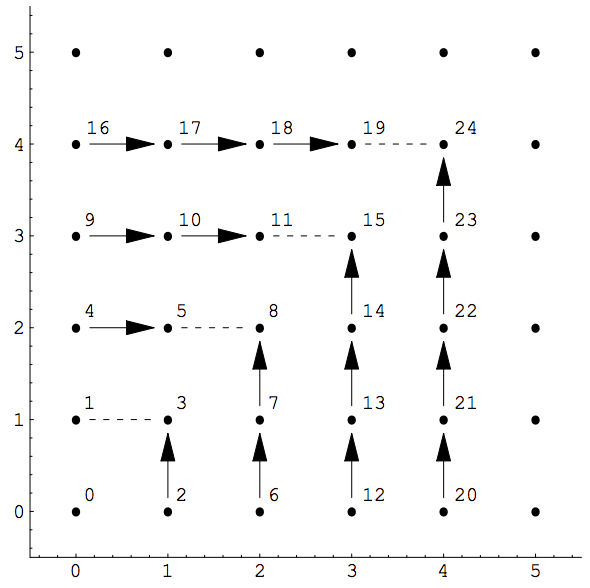
\includegraphics[width=\columnwidth]{Fig-Pairing.png}
  \end{minipage}

  Now please develop a mathematical formula for $\pi'$, (like the notation of original $\pi$),  and prove the correctness of your design.
 
  \begin{solution}
    \begin{displaymath}
    \pi^{'} = \left\{ \begin{array}{ll}
    x + y^2 & \textrm{if $x < y$}\\
    x^2 + x + y & \textrm{otherwise} 
    \end{array} \right.
    \end{displaymath}
  Now we begin to prove that $\pi^{'}$ is bijective. \\
  \textbf{Injective}
  For $\forall (x_1,y_1),(x_2,y_2)$, with $x_1 \ne x_2$ or $y_1 \ne y_2$. We can define $R  =\pi^{'}(x_1,y_1)-\pi^{'}(x_2,y_2)$
  \begin{enumerate}
  \item $x_1 < y_1$ and $x_2<y_2$: $R=(x_1-x_2) + (y_1 -y_2)(y_1 + y_2)$  
  \item $x_1 \le y_1$ and $x_2 \le y_2$: $R=(x_1+x_2+1)(x_1-x_2)+(y_1-y_2)$
  \item $x_1<y_1$ and $x_2 \le y_2$: $R=x_1 + y_1^2 - x_2^2 -x_2 -y_2$.
  \end{enumerate}
    We can infer that none of $R = 0$, thus it is injective. \\
  \textbf{Surjective} For $\forall n \in \mathbb{N}$, $\exists a,b \in \mathbb{N}$, such that $n = a + b^2$. If $a < b$, then we let $x = a$, $y = b$, else if $ a \ge b$, we can let $x = b$, $y = a -b$. That means we fin  That means $\forall n \in \mathbb{N}$, we can find $x$,$y$, makes $\pi^{'}(x,y) = n$. So it is surjective.\\
  
  Therefore the function we desgin is a bijective map form $\mathbb{N}$ to $\mathbb{N}$.
  \end{solution}
 
\end{enumerate}


%========================================================================
\end{document}